\subsubsection{ODEFormer: symbolic regression of continuous-time dynamics}

\citet{dascoli2024odeformer} study \emph{dynamical symbolic regression}. The
observations are samples of one continuous-time trajectory,
$\{(t_i,\mathbf x_i)\}_{i=1}^{N}$, and the symbolic target is the vector field
that governs its instantaneous evolution:

\begin{equation}
\dot{\mathbf x}(t)=\mathbf f(\mathbf x(t)),
\qquad
\mathbf f=(f_1,\ldots,f_{D_{\mathrm{ode}}}):
\mathbb R^{D_{\mathrm{ode}}}\rightarrow
\mathbb R^{D_{\mathrm{ode}}}.
\label{eq:odeformer-vector-field}
\end{equation}

This extends the expression-first principle used by D'Ascoli et al.: first
sample a symbolic mechanism and then execute it to generate observations. The
tree representation remains unary--binary and the target remains a prefix
token sequence. The important change is the meaning of execution. A recurrence
tree directly calculates the next discrete sample; an ODE tree calculates
$\dot{\mathbf x}$ at the current state, and a numerical solver repeatedly
evaluates that tree to produce the observed trajectory.

\paragraph{Sampling a symbolic ODE system.}
The system dimension is sampled uniformly up to
$D_{\mathrm{ode}}=6$. One expression tree is generated independently for each
component $f_k$. For every component, ODEFormer performs the following steps
\citep{dascoli2024odeformer}:

\begin{enumerate}
    \item sample between one and five binary operators and construct a random
    binary-tree shape using the same completion-count procedure used in
    Transformer symbolic-regression generators;

    \item assign addition with probability $3/4$ or multiplication with
    probability $1/4$ to each binary node, and assign a state variable
    $x_j$, $j\in\{1,\ldots,D_{\mathrm{ode}}\}$, to each leaf;

    \item sample between zero and three unary insertions. Each insertion places
    one of $\sin(\cdot)$, $(\cdot)^{-1}$, or $(\cdot)^2$ above a selected
    subtree whose depth remains below six;

    \item add signed coefficients to terms and affine transformations inside
    unary arguments. Their absolute values are sampled log-uniformly between
    $0.05$ and $20$;

    \item serialize $f_1,\ldots,f_{D_{\mathrm{ode}}}$ in prefix notation and
    separate consecutive component equations with a dedicated token
    $\texttt{|}$.
\end{enumerate}

Subtraction is represented by addition with a negative coefficient, while
division is represented by multiplication with an inverse. For example, the
tree

\begin{equation}
f_1(\mathbf x)=a x_1+\sin(bx_2)
\quad\longleftrightarrow\quad
[\texttt{add},\texttt{mul},a,x_1,
  \texttt{sin},\texttt{mul},b,x_2]
\label{eq:odeformer-prefix-example}
\end{equation}

uses exactly the same symbolic objects as functional or recurrent symbolic
regression. Its meaning is now $\dot x_1=f_1(\mathbf x)$.

\begin{figure}[H]
\centering
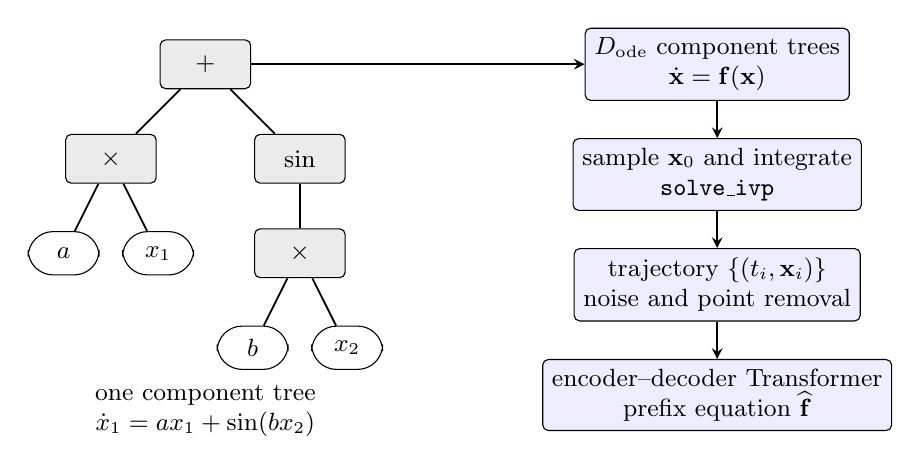
\begin{tikzpicture}[
    operator/.style={draw,rounded corners=2pt,fill=black!8,
        minimum width=1.15cm,minimum height=0.62cm,align=center,font=\small},
    leaf/.style={draw,rounded corners=9pt,fill=white,
        minimum width=0.90cm,minimum height=0.55cm,align=center,font=\small},
    block/.style={draw,rounded corners=2pt,fill=blue!7,
        minimum width=3.15cm,minimum height=0.70cm,align=center,font=\small},
    flow/.style={->,>=stealth,draw,line width=0.7pt},
    branch/.style={draw,line width=0.65pt}
]
    \node[operator] (add) at (-4.4,2.4) {$+$};
    \node[operator] (mul1) at (-5.6,1.2) {$\times$};
    \node[operator] (sin) at (-3.2,1.2) {$\sin$};
    \node[leaf] (a) at (-6.2,0.0) {$a$};
    \node[leaf] (x1) at (-5.0,0.0) {$x_1$};
    \node[operator] (mul2) at (-3.2,0.0) {$\times$};
    \node[leaf] (b) at (-3.8,-1.2) {$b$};
    \node[leaf] (x2) at (-2.6,-1.2) {$x_2$};
    \draw[branch] (add)--(mul1); \draw[branch] (add)--(sin);
    \draw[branch] (mul1)--(a); \draw[branch] (mul1)--(x1);
    \draw[branch] (sin)--(mul2);
    \draw[branch] (mul2)--(b); \draw[branch] (mul2)--(x2);
    \node[font=\small,align=center] at (-4.4,-2.0)
        {one component tree\\$\dot x_1=a x_1+\sin(bx_2)$};

    \node[block] (trees) at (2.1,2.4)
        {$D_{\mathrm{ode}}$ component trees\\$\dot{\mathbf x}=\mathbf f(\mathbf x)$};
    \node[block] (integrate) at (2.1,1.0)
        {sample $\mathbf x_0$ and integrate\\\texttt{solve\_ivp}};
    \node[block] (trajectory) at (2.1,-0.4)
        {trajectory $\{(t_i,\mathbf x_i)\}$\\noise and point removal};
    \node[block] (transformer) at (2.1,-1.8)
        {encoder--decoder Transformer\\prefix equation $\widehat{\mathbf f}$};
    \draw[flow] (add.east) -- (trees.west);
    \draw[flow] (trees)--(integrate);
    \draw[flow] (integrate)--(trajectory);
    \draw[flow] (trajectory)--(transformer);
\end{tikzpicture}
\caption{What remains and what changes in ODEFormer. The symbolic mechanism is
still a unary--binary tree. Numerical integration is inserted between that
tree and the observations because the tree specifies a derivative rather than
the next sample directly.}
\label{fig:odeformer-tree-pipeline}
\end{figure}

\paragraph{From an equation to a training trajectory.}
After sampling $\mathbf f$, the generator draws
$\mathbf x_0\sim\mathcal N(\mathbf 0,\mathbf I)$ and integrates
Equation~\eqref{eq:odeformer-vector-field} from $t=1$ to $t=10$. The number of
stored points $N$ is sampled uniformly from 50 to 200. The implementation uses
SciPy's \texttt{solve\_ivp}, whose default method is adaptive RK45. Failed
integrations and trajectories with $|x_j|>10^2$ are discarded. When every
component becomes nearly constant during the final quarter of the interval,
the example is discarded with probability $0.9$ so that fixed-point solutions
do not dominate the training distribution.

Two corruptions make the observations resemble measurements. A noise scale
$\sigma\sim\mathcal U(0,0.1)$ produces multiplicative Gaussian noise,

\begin{equation}
x_j(t_i)\leftarrow(1+\xi_{i,j})x_j(t_i),
\qquad \xi_{i,j}\sim\mathcal N(0,\sigma^2),
\label{eq:odeformer-noise}
\end{equation}

and a sampled ratio $\rho\sim\mathcal U(0,0.5)$ removes that fraction of time
points uniformly. Consequently, a training pair contains a noisy, irregularly
sampled trajectory as input and the exact prefix representation of the sampled
vector field as target. The formula is retained before integration, so it is
available as mechanism ground truth.

\paragraph{Architecture and inference.}
ODEFormer uses an encoder--decoder Transformer with 86 million parameters, 16
attention heads, and embedding dimension 512. The encoder has four layers and
the decoder has 16. Each timestamp and state value is rounded to four
significant digits and represented by three tokens: sign, mantissa, and
exponent. A feed-forward embedder combines the tokens belonging to one observed
point. Since time is included explicitly in every point, the numerical encoder
uses the timestamps instead of positional embeddings.

The decoder generates the component equations autoregressively in prefix
notation. Beam sampling produces candidate systems; the reported default uses
beam size 50 and temperature 0.1. Every candidate is integrated from the
observed initial condition, and the equation with the highest reconstruction
$R^2$ is selected. An optional BFGS step refines numerical constants. The
complete implementation is released by the authors.\footnote{Official
ODEFormer implementation: \url{https://github.com/sdascoli/odeformer}.}

\paragraph{How mechanism recovery is evaluated.}
The paper distinguishes two trajectory-level tests:

\begin{itemize}
    \item \emph{reconstruction}: integrate $\widehat{\mathbf f}$ from the same
    initial condition and over the same interval used to produce the observed
    trajectory;
    \item \emph{generalization}: integrate $\mathbf f$ and
    $\widehat{\mathbf f}$ from a new initial condition, then compare their
    trajectories over the same time interval.
\end{itemize}

The principal accuracy statistic is the percentage of systems for which the
trajectory $R^2$ exceeds $0.9$. The authors additionally report expression
complexity, defined as the total number of operators, variables, and constants,
and inference time. Generalization is the stronger mechanism-recovery test: two
equations may follow one observed path while generating different dynamics in
other parts of the state space. This also explains why recovering an ODE from
one trajectory is an identifiability problem rather than only a forecasting
problem.

\paragraph{What the recovered ODE explains.}
An explicit ODE gives a global, mechanistic description of the instantaneous
dynamics. For example, the occurrence of $x_j$ in $f_k$ states that variable
$j$ directly participates in the rate of change of variable $k$. This yields a
structural reference

\begin{equation}
M^{\mathrm{GT,ODE}}_{k,j}
=\mathbb I[x_j\text{ occurs in the sampled tree for }f_k].
\label{eq:odeformer-structural-gt}
\end{equation}

A local derivative-level influence can also be calculated from the Jacobian,

\begin{equation}
J_{k,j}(t)=
\left.\frac{\partial f_k(\mathbf x)}{\partial x_j}
\right|_{\mathbf x=\mathbf x(t)}.
\label{eq:odeformer-jacobian}
\end{equation}

These quantities explain which variables govern the \emph{instantaneous rate
of change}. Explaining a finite-horizon state
$\Phi_{\mathbf f}(\Delta;\mathbf x_0)$ requires propagating influence through
the integration. One principled reference is the flow sensitivity

\begin{equation}
\mathbf S(\Delta)=
\frac{\partial\Phi_{\mathbf f}(\Delta;\mathbf x_0)}{\partial\mathbf x_0},
\qquad
\dot{\mathbf S}(t)=
\mathbf J_{\mathbf f}(\mathbf x(t))\mathbf S(t),
\quad \mathbf S(0)=\mathbf I.
\label{eq:odeformer-flow-sensitivity}
\end{equation}

Equations~\eqref{eq:odeformer-structural-gt}--
\eqref{eq:odeformer-flow-sensitivity} are a benchmark interpretation proposed
for this thesis. ODEFormer evaluates reconstructed and generalized trajectories
instead. The distinction resolves the apparent loss of explainability: the
symbolic ODE makes the governing law explicit, while a contribution to a
particular future state additionally depends on the initial condition, the
visited trajectory, interactions, and the chosen horizon.

\paragraph{Position in the proposed research.}
ODEFormer provides a useful advanced extension and a methodological bridge to
continuous-time system identification. The November benchmark can keep its
core around discrete-time recurrences, where a sampled tree directly generates
the next observation and all variable--lag references are immediate. A later
continuous-time module can reuse the same expression-tree interface while
adding initial-condition sampling, numerical integration, solver-failure
filters, and flow-based explanation references. This staging preserves the
main software design while separating the additional numerical and
identifiability challenges of ODE discovery.

